\subsection{Architectural Pattern: Model-View-Controller Structure}
DREAM application can be structured with the Model-View-Controller (MVC) pattern.
The MVC structure consists of three building blocks: model, view, and controller.
\begin{itemize}
    \item the \textbf{Model} provides the methods to access the data useful for the application;
    \item the \textbf{View} displays the real user interface for the presentation of the data contained in the model and deals with the interaction with users;
    \item the \textbf{Controller} receives the user's commands through the view and implements them by accessing the Model and defining the corresponding View to be presented
\end{itemize}

\begin{figure}[H]
  \centering
  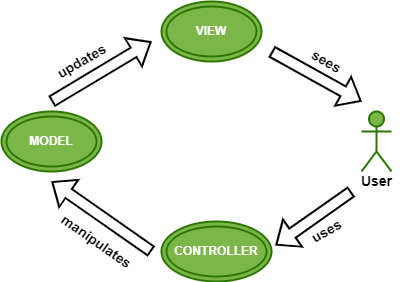
\includegraphics[scale=0.7]{./Images/MVC.png}
  \caption{Model-View-Controller structure}
\end{figure}

This pattern was chosen primarily because application development becomes fast. In fact, it is easier for multiple developers to collaborate and work together given the nature of the architecture itself.
As a result, it also becomes easier to update the application and debug as we have multiple levels properly written in the application.